% Typeset with XeTeX
% Allows use of system fonts rather than just LaTeX's ones
% NOTE - if you use TeXShop and Bibdesk (Mac), can complete citations
%  - open your .bib file, type~\citep{xx... and then F5 or Option-Escape
\documentclass[11pt]{article}
\usepackage[margin=1in, letterpaper]{geometry} % set page layout
%\geometry{letterpaper}  % or a4paper
\usepackage[xetex]{graphicx} % allows us to manipulate graphics.
% Replace option [] with pdftex if you don't use Xe(La)TeX
\usepackage{color}
\usepackage{indentfirst}
\usepackage{hyphenat}
\usepackage{epstopdf} % automatic conversion of eps to pdf 
\usepackage{amsmath, amssymb} % Better maths support & more symbols
\usepackage{textcomp} % provide lots of new symbols - see textcomp.pdf
% line spacing: \doublespacing, \onehalfspacing, \singlespacing
\usepackage{setspace}
\singlespacing
\usepackage{pgfplotstable}
% allows text flowing around figs
% use \begin{wrapfigure}{x}{width} where x = r(ight) or l(eft)
\usepackage{wrapfig}
\usepackage[parfill]{parskip} % don't indent new paragraphs
\usepackage{flafter}  % Don't place figs & tables before their definition 
\usepackage{verbatim} % allows \begin and \end{comment} regions
\usepackage{booktabs} % makes tables look good
\usepackage{bm}  % Define \bm{} to use bold math fonts
% linenumbers in L margin, start & end with \linenumbers \nolinenumbers,
\usepackage{lineno} % use option [modulo] for steps of 5
\usepackage[auth-sc]{authblk} % authors & institutions - see authblk.pdf
%\renewcommand\Authands{ and } % separates the last 2 authors in the list
% control how captions look; here, use small font and indent both margins by 20pt
\usepackage[small]{caption} 
\setlength{\captionmargin}{20pt}

%: FONT
% If you don't want to use system fonts, replace from here to 'Citation style' with \usepackage{Palatino} or similar
%: ************ FANCY FONTS START HERE
\usepackage[no-math]{fontspec} % 'no-math' = keep computer modern for math fonts
\usepackage{xunicode} % needed by XeTeX for handling all the system fonts nicely
\usepackage[no-sscript]{xltxtra} 
\setmonofont[Scale=0.8]{PT Serif} % typeface for \tt commands
\setsansfont[BoldFont={PT Serif Bold}, ItalicFont={PT Serif Italic}]{PT Serif} 
\defaultfontfeatures{Mapping=tex-text}
\setmainfont{Minion Pro}
%\setmainfont{Source Sans Pro}

%: ************ FANCY FONTS END HERE

%:CITATION STYLE
% natbib package: square,curly, angle(brackets)
% colon (default), comma (to separate multiple citations)
% authoryear (default),numbers (citations style)
% super (for superscripted numerical citations, as in Nature)
% sort (orders multiple cites into order of appearance in ref list, or year if authoryear)
% sort&compress: as sort, + multiple citations compressed (as 3-6, 15)
\usepackage[numbers,comma,sort&compress]{natbib}

%:SHORTCUT COMMANDS
% Maths
\newcommand{\ddt}[1]{\ensuremath{\frac{{\rm d}#1}{{\rm d}t}}}  % d/dt
\newcommand{\dd}[2]{\ensuremath{\frac{{\rm d}#1}{{\rm d}#2}}} % dy by dx  - \dd{y}{x}
\newcommand{\ddsq}[2]{\ensuremath{\frac{{\rm d}^2#1}{{\rm d}#2^2}}} % second deriv
\newcommand{\pp}[2]{\ensuremath{\frac{\partial #1}{\partial #2}}} % partial \pp{y}{x}
\newcommand{\ppsq}[2]{\ensuremath{\frac{\partial^2 #1}{\partial {#2}^2}}}
\newcommand{\superscript}[1]{\ensuremath{^{\textrm{#1}}}} %normal (non-math) font for super/subscripts in text
\newcommand{\subscript}[1]{\ensuremath{_{\textrm{#1}}}}
\newcommand{\positive}{\ensuremath{^+}}
\newcommand{\negative}{\ensuremath{^-}}
% Editing
\newcommand{\red}[1]{{\color{red}{#1}}}
\newcommand{\redtext}[1]{{\color{red}{#1}}}
\newcommand{\blue}[1]{{\color{blue}{#1}}}
\newcommand{\bluetext}[1]{{\color{blue}{#1}}}
\newcommand{\scinot}[2]{\ensuremath{#1 \times 10^{#2}}}
% Standard stuff
\newcommand{\be}{\begin{equation}}
\newcommand{\ee}{\end{equation}}
\newcommand{\bea}{\begin{eqnarray}}
\newcommand{\eea}{\end{eqnarray}}
\newcommand{\ie}{\textit{i.e.}}
\newcommand{\etal}{\textit{et al.}}
\newcommand{\khi}{Ki67$^\text{hi}$}
\newcommand{\klo}{Ki67$^\text{lo}$}


% \begin{graybox} text \end{graybox} for text with a background colour
\definecolor{MyGray}{rgb}{0.96,0.97,0.98}
\definecolor{MyGray}{rgb}{0.96,0.90,0.98}
\makeatletter\newenvironment{graybox}{%
	\begin{lrbox}
		{\@tempboxa}\begin{minipage}[r]{0.98\columnwidth}}{\end{minipage}\end{lrbox}%
	\colorbox{MyGray}{\usebox{\@tempboxa}}
}\makeatother


%%%%%%%%%%%%%%%%%%%%%%%

\title{Supplementary Information}
\author{}

\date{}

\begin{document} 
	\maketitle
	
\vspace{-2cm}
\section{Methods}
\subsection{Analysing and selecting mathematical models using Bayesian Approach.}

We attempted to describe the kinetics of host and donor cells in busulfan chimeric mice using an array of mathematical models (described in section $\ref{models}$).
Due to variation in the degree of depletion  of host HSCs by busulfan treatment, the level at which the fraction of donor cells stabilize in each subset varies across mice.
We address this issue by normalising the donor fractions in any given B cell subsets to the donor fractions in the upstream precursor populations. We refer to this as the normalized chimerism:
\vspace{-2mm}
$$
f_\text{d} = \frac{\text{Donor counts}}{\text{Total counts} \times \chi},  \quad \text{where } \chi \text{ is the fraction of cells in the precursor population that are donor-derived.}
$$
This allows us to fit a single model to data from multiple mice, that may have responded differently to busulfan treatment.
Each model was fitted simultaneously to the total cell counts ($N$, the sum of host and donor cells), the normalised donor fraction ($f_{d}$) and the proportions of \khi cells ($\kappa$) in the host and donor compartments.
Cell counts were log-transformed while $f_{d}$ and $\kappa$ were transformed using the \textit{logit} function to ensure that measurement errors were normally distributed.
  
We then used the Bayesian approach to estimate the model parameters,  the errors associated with the measurements in each dataset, and a measure of the support for the model.  The inputs to this procedure are (i) an expression for the joint likelihood of the data, in terms of the model parameters and the (unknown) errors associated with each dataset; and (ii) a set of distributions on both the model parameters and the magnitude of the measurement errors in each dataset, representing any insights we may have regarding their values and referred to as \textit{priors}.  The Bayesian procedure updates these priors with the likelihood, to generate posterior distributions that reflect our knowledge of these parameters in the light of the data. Strong (narrow)  priors  help to \textit{regularise} a model's behaviour and prevent it from learning too much from the data -- and hence guard against over-fitting. 
 
The \textit{posterior} distribution of parameters ($\theta_{\text{post}}$) for a given model is estimated using Bayes' rule, 
\be
p(\theta_{\text{post}} | y) = \frac{p(y |\theta_{\text{post}})\, . \, p(\theta_{\text{prior}})}{p(y)} 
\ee
where $p(y)$ is the  \textit{likelihood} of the data (averaged over the \textit{priors}) that normalises the \textit{posterior} such that it integrates to 1. 
In our analysis, \textit{priors} are considered to be tools that improve model's ability to learn from the data and are subjected to similar standards of evaluation and revaluation like any other component of the model.

Our each model is represented as a system of ordinary differential equations (ODEs, described in details in section \ref{models}), which is solved numerically using the `\textit{integrate\_ode\_rk45}' solver available in \textit{Stan} programming language.
During an individual iteration of the fitting  process, a set of parameter values are drawn from $\theta_{\text{prior}}$ repeatedly using a MCMC based \textit{NUTS} sampler, in order to provide probable predictions of the combined data and calculate the joint \textit{likelihood}.   
The generalised strategy that we use for Bayesian analysis is depicted below. Model specific details of \textit{prior} distributions of parameters are described in their respective paragraphs in section $\ref{models}$.

We assumed that the suitably transformed measurements of total cell counts,normalised chimerism and proportions of {\khi} cells in host and donor compartments were all normally distributed with unknown but constant errors at each time point,
\be
\begin{aligned}
N &\sim \text{Normal}(\mu_N, \sigma_N), \\
f_d &\sim \text{Normal}(\mu_{fd}, \sigma_{fd}),\\
\kappa_{\text{host}} &\sim \text{Normal}(\mu_{\kappa_{\text{host}}}, \sigma_{\kappa_{\text{host}}}),\\
\kappa_{\text{donor}} &\sim \text{Normal}(\mu_{\kappa_{\text{donor}}}, \sigma_{\kappa_{\text{donor}}}).
\end{aligned}
\ee
Here, $\mu$ is the mean of model predictions estimated by averaging the model predictions across the whole \textit{posterior} distribution weighted by the \textit{likelihood} of data at a given time-point.\\
The standard deviation $\sigma$ indicates the uncertainty in $\mu$, which is estimated from the model fits. 
The \textit{R-stan} package in \textit{R} software is used to interface and compile the code written for model definitions, sampling and fitting procedures in \textit{stan} programming language. 

\subsection*{Model comparisons}

We evaluate the mathematical models studied here in two separate ways.
First by running posterior-predictive checks on the same data that was used for fitting procedures and second by estimating the out-of-sample prediction error i.e the ability of the model to accurately predict new data. 

Posterior-predictive checks involve replicating data ($y^{rep}$) by simulating the fitted model using the posterior distribution of parameters and comparing that to the observed data ($y^{obs}$).
Since, we use the whole \textit{posterior}, these checks include the uncertainty associated with parameter estimations, which is an advantage over non-bayesian methods.  
Posterior-predictive check helps assess the validity of the model by displaying systematic discrepancies between $y^{rep}$ and $y^{obs}$ and therefore works as a diagnostic tool in rebuilding the model.
\red{Its just a systematic way to ask whether your model makes sense in the light of observed data.}

We then estimate the out-of-sample prediction error which is slightly more complicated and computationally expensive.
First the log predictive density $\text{log}\big(p(y|\theta)\big)$ (also called as the log-likelihood) of the given observation is estimated by simulating `D' number draws from the posterior distribution for the fitted model. 
The whole process is repeated for each data point ($y_1,... , y_n$) to calculate log point-wise predictive density (\textit{lppd}) as described in eq.\ref{eq:lppd}.
Then the out-of-sample prediction error is estimated using the method of cross-validation, where data is divided into (i) a training sample ($y_{\text{train}}$), which is used to fit the model and (ii) a test sample ($y_{\text{test}}$), which is used to evaluate the predictive accuracy of the model.
\be
\text{lppd} = \sum_{i=1}^{n} \, \text{log} \bigg(\frac{1}{D} \sum_{d=1}^{D} \, p(y_i | \theta_{\text{post}}^d) \bigg)
\label{eq:lppd}
\ee
%Classically, deviance has been considered as the measure of predictive accuracy of the model which is -2 times the log predictive density at the point estimate of parameters ($\hat{\theta}$).
The advantage of using \textit{lppd} over deviance is that it measures the difficulty in predicting observations at each unique point in the data and thus provides more accurate descriptions of the uncertainty in model predictions.
Additionally we use a special case of cross-validation called `leave-one-out' (\textit{loo}) method to compute the out-of-sample prediction error, which substantially minimises the problem of over-fitting. \red{(i.e. model learning too much from the data).}
In this method, a dataset of size `n' ($y_1,... , y_n$) is partitioned into `n' number of samples such that each test sample contains a single observation. 
%Model's ability to predict the `left-out' observation in the test sample is evaluated based on its fit to the training sample that contains remaining (n-1) observations.
The model is fitted on the training set containing (n-1) observations and is tested for the prediction accuracy of the `left-out' observation. 
This process is repeated for all the elements in the test sample and the out-of-sample prediction error is estimated by simulating `D' number draws from the posterior distribution.
The \textit{loo} estimate of lppd is therefore the summed value of the log-predictive densities calculated for each element in test sample from the posterior draws fitted on the observations excluding the test sample. 
 (eq.\ref{eq:lppd-loo}).
\be
\begin{aligned}
\text{lppd}^{loo} &= \sum_{i=1}^{n} \, \text{log} \,\, p(y_i | \theta_{\text{post}}^{(\text{-}i)}) \\
                  &= \sum_{i=1}^{n} \, \text{log} \,\,  \bigg(\frac{1}{D} \sum_{d=1}^{D} \, p(y_i | \theta_{\text{post}}^{(\text{-}i)d}) \bigg)
\end{aligned}
\label{eq:lppd-loo}
\ee
Where $\theta_{\text{post}}^{(\text{-}i)d}$ characterizes D posterior simulations fitted on (n-1) observations when i$^{th}$ observation is left out.
%[Andrew Gelman, Jessica Hwang, and Aki Vehtari,  Statistics and Computing, Nov 2014]

We use the \textit{loo-2.0} package in \textit{R} to calculate the lppd$^{loo}$ estimates for each model. 
The \textit{loo-2.0} package uses Pareto-smoothed importance sampling (PSIS), which is an approximation of \textit{loo} cross-validation that uses existing posterior draws from the model fits to estimate the lppd$^{loo}$ values (Vehtari et al, Statistics and Computing, Aug 2016).

The lppd$^{loo}$ estimate by itself does not provide any information about model's suitability to the data.
However, it can be used to rank different models, such that the model with lowest lppd$^{loo}$ value has the highest support.
It is also used to calculate \textit{Akaike weight}, which is the probability that a given model will explain new data better as compared to all the other models considered in the analysis.  
We estimate \textit{Akaike weights} by exponentiating the negative half of $\Delta$lppd$^{loo}$ (i.e the difference between each lppd$^{loo}$ and the lowest lppd$^{loo}$) value and then standardise it by dividing by the total value for `M' number of models. (eq.~\ref{eq:akaike_weights}).
\be
Aw_i = \frac{\text{exp}(-\frac{1}{2}\, \Delta \text{lppd}^{loo}_i)}{\sum_{m=1}^{M} \,\text{exp}(-\frac{1}{2}\, \Delta \text{lppd}^{loo}_m) }
\label{eq:akaike_weights}
\ee


\clearpage
\subsection{Modelling the dynamics of chimerism in the precursor population}
%The quantity, normalised donor fraction $f_{d}$, is independent of chimerism and is only sensitive to parameters that are common across animals.
We describe the changes in chimerism in the source populations over time using a phenomenological function (equation~\ref{eq:source_chimerism}) that reasonably depicts the shape of the timecourse of fraction of donor cells across all animals.
\be
\chi(t) = \chi_{stable} \, (1 - e^{-q \,t}) 
\label{eq:source_chimerism}
\ee
Parameters `$\chi_{stable}$' and `q' are estimated by fitting the spline in equation~\ref{eq:source_chimerism} to the observed donor fractions in the source compartment.

\begin{figure}[htbp]
	\centerline{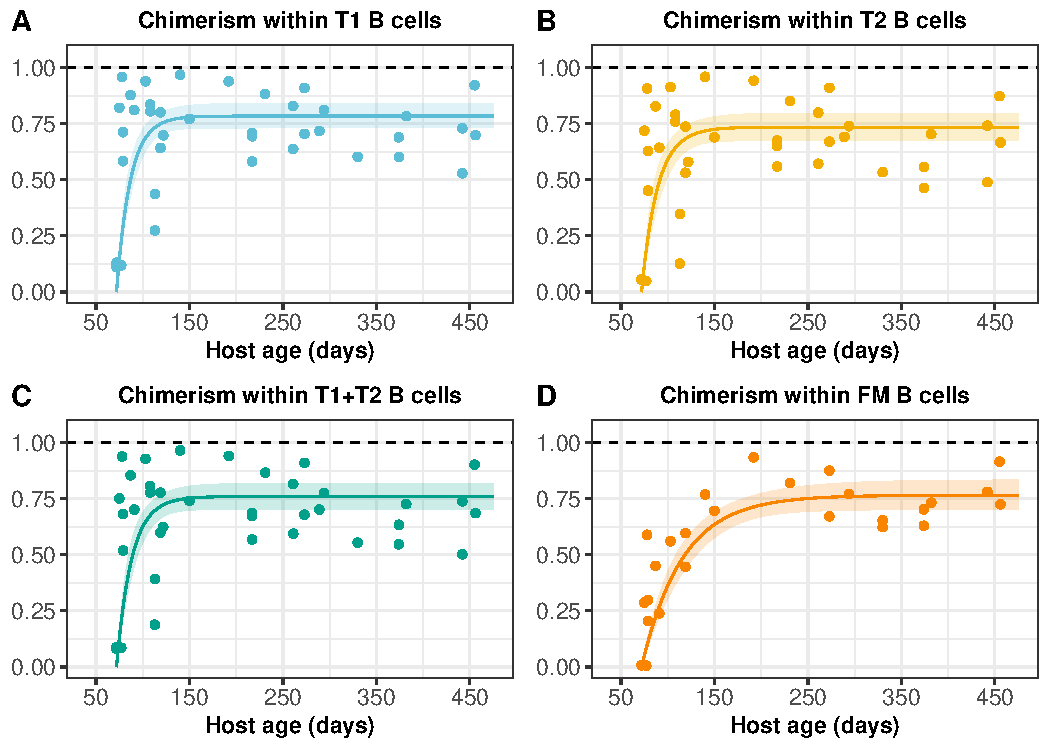
\includegraphics[scale = 0.85] {SI_source_chimerism.pdf}}
	\caption{ \textbf{The time-course of absolute chimerism within precursor compartments.} Solid lines indicate the most probable description of changes in the chimerism with host age, modelled according to equation~\ref{eq:source_chimerism}. Shaded envelopes denote the uncertainty in the most probable prediction and are drawn by taking 4.5 and 95.5 percentiles intervals of model predictions made from the posterior distribution of parameters.}
	\label{fig:source_chi}
\end{figure}

\subsection{Modelling Source influx} \label{source_influx}
We assumed that the rate of influx from source $\psi$, stays constant and used the size of the source compartment as a proxy to estimate the number of cells maturing into the target pool.  
Equation~\ref{eq:source_counts}, is a spline that is used to describes the changes in the source over time. 
Parameters $S_0$ and $\nu$ are estimated by fitting the spline in equation~\ref{eq:source_counts} to the observed cell counts in the source compartment.
\be
S(t) = S_0 \, e^{-\nu \, t}
\label{eq:source_counts}
\ee
The proportion of source population entering the target pool ($\psi$) is assumed to remains constant over time and is estimated from the model fits.
Daily source influx into FM and GC populations is therefore given by equation~\ref{eq:influx},
\bea
\begin{aligned}
	&\phi(t) = \psi \, S(t), \\
	&\phi_{\text{donor}}(t) = \psi \, S(t) \, \chi(t),  \\
	&\phi_{\text{host}}(t) = \phi(t) - \phi_{\text{donor}}(t).
\end{aligned}
\label{eq:influx}
\eea
We also explored variant of our models in which $\psi$ varied with time ($\psi(t)=\psi_0\,e^{p\,t}$), which failed to improve on the quality of fits that we received with constant $\psi$.
Parameters $\psi_0$ and `p' are estimated from model fits to the time-course of total counts, normalised chimerism and \khi fractions of the target population. 

\begin{figure}[htbp]
	\centerline{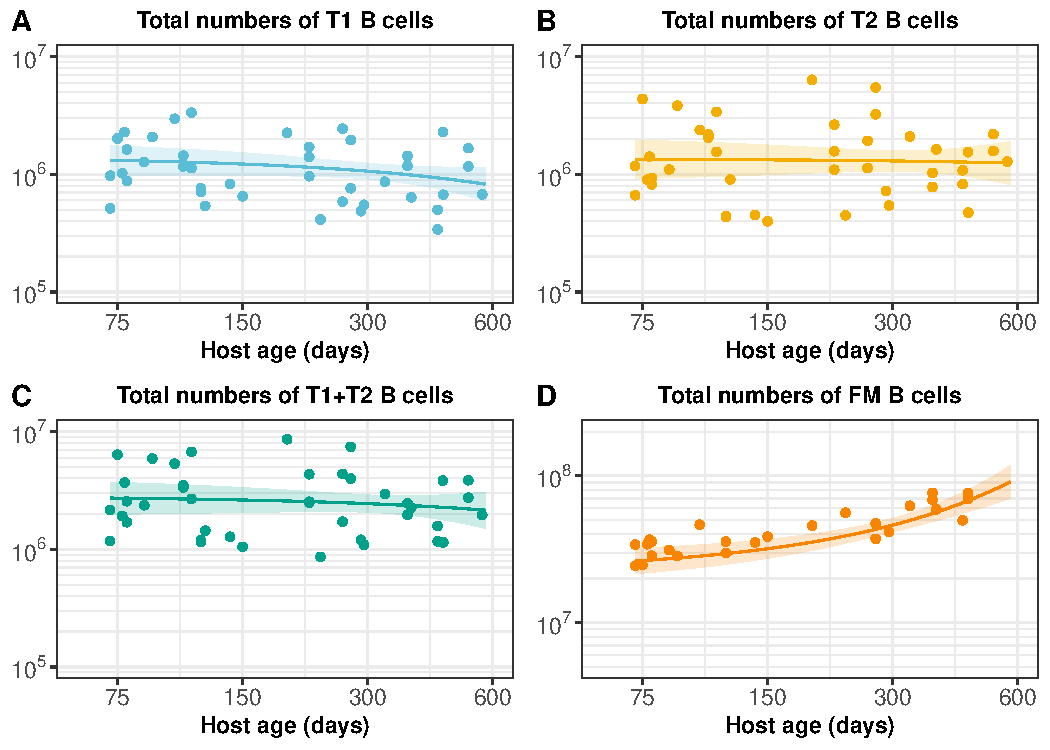
\includegraphics[scale = 0.85] {SI_source_counts.pdf}}
	\caption{ \textbf{The time-course of total counts of precursor compartments.} Solid lines indicate the most probable description of changes in the size of the precursor population with host age, modelled according to equation~\ref{eq:source_counts}. Shaded envelopes denote the uncertainty in the most probable prediction and are drawn by taking 4.5 and 95.5 percentiles intervals of model predictions made from the posterior distribution of parameters.}
	\label{fig:source_counts}
\end{figure}
\clearpage


\subsection{Mathematical models used to describe B cell population dynamics} $\label{models}$
\vspace{-1cm}
\paragraph*{Simple homogeneous model:}
%\textit{All cells behave identically at all times.} \\
In this model we assume that cells follow random birth-death processes to form a kinetically homogeneous population that self renews through homoeostatic division ($\rho$) and decays by death and maturation. 
We define the rate of cellular turnover `$\delta$', which accounts for combined loss of cells by death and by differentiation events.  
%Per capita net loss rate `$\lambda$' is therefore given by turnover - proliferation ($\delta - \rho$) and is constant in this model.
Influx of cells from the source compartment is given by $\phi$ and is modelled as shown in section \ref{source_influx}. 
We model the dynamics of \khi $(Y)$ and \klo $(X)$ cells using the coupled system of ODEs depicted below,
\bea
\begin{aligned}
\dot Y(t) &= \phi(t) \epsilon \, + \rho \,(2 \, X(t) + Y(t)) - (\beta + \delta) \, Y(t),\\
\dot X(t) &= \phi(t) (1-\epsilon) \, + \beta  \, Y(t) - (\rho + \delta) \, X(t).
\label{eq:SHM}
\end{aligned}
\eea
Here, $\beta$ is the rate of loss of Ki67 expression after mitosis, which is estimated form the model fits and $\epsilon$ denotes the proportion of the cells entering from source that are \khi, which is calculated from observations and used as an input in the model fitting process.

We define time `$t_0$' as the age at BMT of the youngest recipient.
The proportions of \khi cells in the host compartment at $t_0$ \big($\kappa_{\text{host}}(0) = \kappa_0$\big), are estimated from the model fits. 
At the time of BMT, the size of donor compartment is zero \ie $N_{\text{donor}} = 0$.
Therefore, the proportions of \khi cells in the donor compartment at $t_0$ would reflect the proportions of \khi cells in the source influx \ie \, $\kappa_{\text{donor}}(0) = \epsilon$. 
The initial sizes of \khi and \klo subsets within the host compartment are therefore given as $N_0 \, \kappa_0$ and $N_0 \, (1 - \kappa_0)$, respectively. 

%: Table 3
\begin{table}[h!]
	\begin{center}
	\textbf{Priors on the model parameters for the Simple homogeneous model}\\
		\renewcommand{\arraystretch}{1.2}
		\begin{tabular}{l l l l l } 
			\toprule 
			\textbf{Unknowns}              &                                     & \textbf{FM}           & \textbf{Spleen GC}        &  \textbf{LN GC}        \\ 
			\toprule
			\textbf{Parameters}            &$\psi$ ($\ge$ 0) ($\le$ 1)           & Normal(0.5, 0.25)     & Normal(0.001, 0.5)   &  Normal(0.001, 0.5)   \\ 			                               
			                               &$\rho$ ($\ge$ 0)                     & Normal(0.01, 0.5)     & Normal(0.01, 0.5)    &  Normal(0.01, 0.5)    \\
			                               &$\delta$ ($\ge$ 0)                   & Normal(0.01, 0.5)     & Normal(0.01, 0.5)    &  Normal(0.01, 0.5)    \\
			                               &$\beta$ ($\ge$ 0)                    & Normal(3.5, 1)        & Normal(3.5, 1)       &  Normal(3.5, 1) \\
			                               &&&&\\
			\textbf{Initial conditions}    &log($N_0$)                           & Normal(17, 1)         & Normal(11, 1)        &  Normal(11, 0.4)      \\			                               
			                               &$\kappa_0$ ($\ge$ 0) ($\le$ 1)       & Normal(0.2, 0.15)     & Normal(0.9, 0.05)    &  Normal(0.9, 0.05)    \\
			                               &&&&\\
			\textbf{Variance}              &$\sigma_N$ ($\ge$ 0)                 & Cauchy(1, 1)          & Cauchy(0.7, 1)       &  Cauchy(0.3, 0.5)     \\ 
		                               	   &$\sigma_{fd}$ ($\ge$ 0)              & Cauchy(1.5, 1)        & Cauchy(0.2, 1)       &  Cauchy(0.4, 0.5)     \\
			                               &$\sigma_{\kappa_{donor}}$ ($\ge$ 0)  & Cauchy(1, 1)          & Cauchy(0.05, 1)      &  Cauchy(0.9, 0.5)     \\ 
			                               &$\sigma_{\kappa_{host}}$ ($\ge$ 0)   & Cauchy(0.5, 1)        & Cauchy(0.05, 1)      &  Cauchy(0.5, 0.5)     \\
			\hline
			\toprule 
		\end{tabular}
	\end{center}
	\label{tab:priors_cbdm}
\end{table} 

\paragraph*{Time-dependent model:} 
%\textit{All cells behave identically at a given instant of time.} \\
This is a homogeneous model where the fitness of a population, defined as its ability to grow either by enhanced cellular division ($\rho$) or decreased turnover ($\delta$), varies with time.
However, at any given instant of time all cells in the population behave identically. % obey the same rules of turnover and division.
%We assume that the fitness of the whole population varies over time, due to changes in their environment. 
Variation in the fitness may be a result of changes in the cellular environment manifested as animals age.
We explored different forms of either rates of cell division ($\rho$) or turnover ($\delta$) changing with time and the best-fit was obtained when turnover declines exponentially with host age ($\delta_0 \, e^{-r\,t}$) while the rate of division remains unaltered.
\bea
\begin{aligned}
	\dot Y(t) &= \phi(t) \epsilon \, + \rho(t) \,(2 \,  X(t) + Y(t)) - (\beta + \delta(t)) \, Y(t),\\
	\dot X(t) &= \phi(t) (1-\epsilon) \, + \beta  \, Y(t) - (\rho(t) + \delta(t)) \, X(t).
	\label{eq:TDM}
\end{aligned}
\eea
%: Table 4
\begin{table}[h!]
	\begin{center}
		\textbf{Priors on the model parameters for the Time-dependent model}\\
		\renewcommand{\arraystretch}{1.2}
		\begin{tabular}{l l l l l } 
			\toprule 
			\textbf{Unknowns}              &                                     & \textbf{FM}           & \textbf{Spleen GC}        &  \textbf{LN GC}        \\ 
			\toprule
			\textbf{Parameters}            &$\psi$ ($\ge$ 0) ($\le$ 1)           & Normal(0.5, 0.25)     & Normal(0.001, 0.5)   &  Normal(0.001, 0.5)   \\ 			                               
			&$\rho$ ($\ge$ 0)                     & Normal(0.01, 0.5)       & Normal(0.01, 0.5)    &  Normal(0.01, 0.5)    \\
			&$\delta_0$ ($\ge$ 0)                 & Normal(0.01, 0.5)       & Normal(0.01, 0.5)    &  Normal(0.01, 0.5)    \\
			&$r   $                               & Normal(0, 0.3)          & Normal(0, 0.3)       &  Normal(0, 0.3)       \\
			&$\beta$ ($\ge$ 0)                    & Normal(3.5, 1)          & Normal(3.5, 1)       &  Normal(3.5, 1)       \\
			&&&&\\
			\textbf{Initial conditions}    &log($N_0$)                           & Normal(17, 1)         & Normal(11, 1)        &  Normal(11, 0.4)      \\			                               
			&$\kappa_0$ ($\ge$ 0) ($\le$ 1)       & Normal(0.2, 0.15)     & Normal(0.9, 0.05)    &  Normal(0.9, 0.05)    \\
			&&&&\\
			\textbf{Variance}              &$\sigma_N$ ($\ge$ 0)                 & Cauchy(1, 1)          & Cauchy(0.7, 1)       &  Cauchy(0.3, 0.5)     \\ 
			&$\sigma_{fd}$ ($\ge$ 0)              & Cauchy(1.5, 1)        & Cauchy(0.2, 1)       &  Cauchy(0.4, 0.5)     \\
			&$\sigma_{\kappa_{donor}}$ ($\ge$ 0)  & Cauchy(1, 1)          & Cauchy(0.05, 1)      &  Cauchy(0.9, 0.5)     \\ 
			&$\sigma_{\kappa_{host}}$ ($\ge$ 0)   & Cauchy(0.5, 1)        & Cauchy(0.05, 1)      &  Cauchy(0.5, 0.5)     \\
			\hline
			\toprule 
		\end{tabular}
	\end{center}
	\label{tab:priors_tdm}
\end{table} 

\paragraph{Kinetic-heterogeneity model:}
%\textit{This is also a heterogeneous model} \\
This model assumes that the given population is heterogeneous, composed of kinetically distinct subsets that turnover or divide at different rates. 
The subset with faster kinetics of net loss  would get replaced quickly new cells coming form the source, while the one with slower kinetics would resist the replacement.
As a result, we expect a sharp increase in the donor fraction initially which then stabilises slowly to the level of donor faction in the source compartment.
\be
\begin{aligned}
\dot Y_f(t) &= \phi(t) \, f \, \epsilon \, + \rho_f \,(2 \, X_f(t) + Y_f(t)) - (\beta + \delta_f) \, Y_f(t),\\
\dot X_f(t) &= \phi(t) \, f \, (1-\epsilon) \, + \beta  \, Y_f(t) - (\rho_f + \delta_f) \, X_f(t), \\
\dot Y_s(t) &= \phi(t) \, (1-f) \, \epsilon \, + \rho_s \,(2 \, X_s(t) + Y_s(t)) - (\beta + \delta_s) \, Y_s(t),\\
\dot X_s(t) &= \phi(t) \, (1-f) \, (1-\epsilon) \, + \beta  \, Y_s(t) - (\rho_s + \delta_s) \, X_s(t).
\end{aligned}
\label{eq:KHM}
\ee
We assume that fast and slow subsets exist in both host and donor sub-populations and therefore solve the ODEs depicted in eq.~\ref{eq:KHM} separately for each compartment.
$f$ and $\alpha$ are the proportions of fast subset in the source and the target population, respectively. 
Initial sizes of the fast and slow subsets within the host compartment are given as $N_0 \, \alpha$ and $N_0 \, (1 -\alpha)$, respectively.
The initial fraction of \khi cells ($\kappa_0$) in fast and slow subsets were allowed to be different and were estimated

%: Table 5
\begin{table}[h!]
	\begin{center}
		\textbf{Priors on the model parameters for the Kinetic heterogeneity model}\\
		\renewcommand{\arraystretch}{1.2}
		\begin{tabular}{l l l l l } 
			\toprule 
			\textbf{Unknowns}              &                                     & \textbf{FM}           & \textbf{Spleen GC}        &  \textbf{LN GC}        \\ 
			\toprule
			\textbf{Parameters}            &$\psi$ ($\ge$ 0) ($\le$ 1)           & Normal(0.5, 0.25)     & Normal(0.001, 0.5)   &  Normal(0.001, 0.5)   \\ 			                               
			&$\rho_{\text{fast}}$ ($\ge$ 0)                     & Normal(0.01, 0.5)     & Normal(0.01, 0.5)    &  Normal(0.01, 0.5)    \\
			&$\delta_{\text{fast}}$ ($\ge$ 0)                   & Normal(0.01, 0.5)     & Normal(0.01, 0.5)    &  Normal(0.01, 0.5)    \\
			&$\rho_{\text{slow}}$ ($\ge$ 0)                     & Normal(0.01, 0.5)     & Normal(0.01, 0.5)    &  Normal(0.01, 0.5)    \\
			&$\delta_{\text{slow}}$ ($\ge$ 0)                   & Normal(0.01, 0.5)     & Normal(0.01, 0.5)    &  Normal(0.01, 0.5)    \\
			&$\beta$ ($\ge$ 0)                     & Normal(3.5, 1)        & Normal(3.5, 1)       &  Normal(3.5, 1)       \\
			&$f$ ($\ge$ 0) ($\le$ 1)              & Normal(0.05, 0.25)     & Normal(0.05, 0.5)   &  Normal(0.05, 0.5)   \\ 	
			&&&&\\
			\textbf{Initial conditions}    &log($N_0$)                           & Normal(17, 1)         & Normal(11, 1)        &  Normal(11, 0.4)      \\			                               
			&$\alpha$ ($\ge$ 0) ($\le$ 1)           & Normal(0.5, 0.25)     & Normal(0.5, 0.25)   &  Normal(0.5, 0.25)   \\
			&$\kappa_\text{Fast}(0)$ ($\ge$ 0) ($\le$ 1)       & Normal(0.2, 0.15)     & Normal(0.9, 0.05)    &  Normal(0.9, 0.05)    \\
			&$\kappa_\text{slow}(0)$ ($\ge$ 0) ($\le$ 1)       & Normal(0.2, 0.15)     & Normal(0.9, 0.05)    &  Normal(0.9, 0.05)    \\
			&&&&\\
			\textbf{Variance}              &$\sigma_N$ ($\ge$ 0)                 & Cauchy(1, 1)          & Cauchy(0.7, 1)       &  Cauchy(0.3, 0.5)     \\ 
			&$\sigma_{fd}$ ($\ge$ 0)              & Cauchy(1.5, 1)        & Cauchy(0.2, 1)       &  Cauchy(0.4, 0.5)     \\
			&$\sigma_{\kappa_{donor}}$ ($\ge$ 0)  & Cauchy(1, 1)          & Cauchy(0.05, 1)      &  Cauchy(0.9, 0.5)     \\ 
			&$\sigma_{\kappa_{host}}$ ($\ge$ 0)   & Cauchy(0.5, 1)        & Cauchy(0.05, 1)      &  Cauchy(0.5, 0.5)     \\
			\hline
			\toprule 
		\end{tabular}
	\end{center}
\label{tab:priors_khm}
\end{table} 


\paragraph{Incumbent model:}
%\textit{This is also a heterogeneous model} \\
The incumbent model (Hogan et al PNAS 2015 and Rane et al PLoS Bio 2018) is the variant of kinetic-heterogeneity model which assumes that heterogeneity is exhibited only in the host compartment.
All donor cells follow the same rules of turnover and division in this model.
Whereas the host compartment is composed of - (i) an incumbent subset of older, self-renewing cells that are resistant to displacement by new cells and (ii) a dis-placeable subset that turns over with a constant net loss rate `$\lambda$' and is replaced continuously by cohorts of new cells entering the pool.
\be
\begin{aligned}
\dot Y(t) &= \phi(t) \epsilon \, + \rho \,(2 \, X(t) + Y(t)) - (\beta + \delta) \, Y(t),\\
\dot X(t) &= \phi(t) (1-\epsilon) \, + \beta  \, Y(t) - (\rho + \delta) \, X(t), \\
\dot Y_{\text{inc}}(t) &=  \rho_{\text{inc}} \,(2 \, X_{\text{inc}}(t) + Y_{\text{inc}}(t)) - (\beta + \delta_{\text{inc}}) \, Y_{\text{inc}}(t),\\
\dot X_{\text{inc}}(t) &=  \beta  \, Y_{\text{inc}}(t) - (\rho_{\text{inc}} + \delta_{\text{inc}}) \, X_{\text{inc}}(t).
\end{aligned}
\label{eq:INC}
\ee
We assume that the incumbent subset is established very early in the mouse life and hence could only be present in the host compartment, since the minimum age of BMT in chimeric animals was $\sim$7 weeks. 

%: Table 6
\begin{table}[h!]
	\begin{center}
		\textbf{Priors on the model parameters for the Incumbent model}\\
		\renewcommand{\arraystretch}{1.2}
		\begin{tabular}{l l l l l } 
			\toprule 
			\textbf{Unknowns}              &                                     & \textbf{FM}           & \textbf{Spleen GC}        &  \textbf{LN GC}        \\ 
			\toprule
			\textbf{Parameters}            &$\psi$ ($\ge$ 0) ($\le$ 1)           & Normal(0.5, 0.25)     & Normal(0.001, 0.5)   &  Normal(0.001, 0.5)   \\ 			                               
			&$\rho$ ($\ge$ 0)                     & Normal(0.01, 0.5)     & Normal(0.01, 0.5)    &  Normal(0.01, 0.5)    \\
			&$\delta$ ($\ge$ 0)                   & Normal(0.01, 0.5)     & Normal(0.01, 0.5)    &  Normal(0.01, 0.5)    \\
			&$\rho_{\text{inc}}$ ($\ge$ 0)                     & Normal(0.01, 0.5)     & Normal(0.01, 0.5)    &  Normal(0.01, 0.5)    \\
			&$\delta_{\text{inc}}$ ($\ge$ 0)                   & Normal(0.01, 0.5)     & Normal(0.01, 0.5)    &  Normal(0.01, 0.5)    \\
			&$\beta$ ($\ge$ 0)                     & Normal(3.5, 1)        & Normal(3.5, 1)       &  Normal(3.5, 1)       \\
			&&&&\\
			\textbf{Initial conditions}    &log($N_0$)                           & Normal(17, 1)         & Normal(11, 1)        &  Normal(11, 0.4)      \\			                               
			&$\alpha$ ($\ge$ 0) ($\le$ 1)           & Normal(0, 0.25)     & Normal(0, 0.25)   &  Normal(0, 0.25)   \\
			&$\kappa_0$ ($\ge$ 0) ($\le$ 1)       & Normal(0.2, 0.15)     & Normal(0.9, 0.05)    &  Normal(0.9, 0.05)    \\
			&$\kappa_\text{inc}(0)$ ($\ge$ 0) ($\le$ 1)       & Normal(0.2, 0.15)     & Normal(0.9, 0.05)    &  Normal(0.9, 0.05)    \\
			&&&&\\
			\textbf{Variance}              &$\sigma_N$ ($\ge$ 0)                 & Cauchy(1, 1)          & Cauchy(0.7, 1)       &  Cauchy(0.3, 0.5)     \\ 
			&$\sigma_{fd}$ ($\ge$ 0)              & Cauchy(1.5, 1)        & Cauchy(0.2, 1)       &  Cauchy(0.4, 0.5)     \\
			&$\sigma_{\kappa_{donor}}$ ($\ge$ 0)  & Cauchy(1, 1)          & Cauchy(0.05, 1)      &  Cauchy(0.9, 0.5)     \\ 
			&$\sigma_{\kappa_{host}}$ ($\ge$ 0)   & Cauchy(0.5, 1)        & Cauchy(0.05, 1)      &  Cauchy(0.5, 0.5)     \\
			\hline
			\toprule 
		\end{tabular}
	\end{center}
	\label{tab:priors_inc}
\end{table} 


\end{document}



